%!TEX root = ../Master.tex

\section{System setup and scenario}\label{sec:methodmaterials}

The system examined in this paper is illustrated in Figure \ref{fig:usecase}. It consists of a drone-based sender that is able to adjust three mechanisms to obtain reliability: the TxR, the amount of redundancy introduced by RLNC and the video rate. We base the adaptation of the three mechanisms on the PER. This limits our policy to a single feedback measure, which has three advantages (i) it results in a simple policy, (ii) it does not require specialized equipment at the receivers and (iii) it is easy to compare the conditions at multiple receivers. The adjustment of the mechanisms, depicted in Figure \ref{fig:usecase}, is the following: 1) the sender receives information about the PER, which is made available to both the TxR and the RLNC component; 2) based on the PER information, the transmitter follows a decision policy to change the redundancy and TxR; 3) the video rate component is notified of the remaining data available and adjusted accordingly; 4) video data is delivered to the RLNC component and redundancy is added; 5) the coded packets are transmitted with the rate determined by the TxR component.
\begin{figure}[ht]
  \centering
  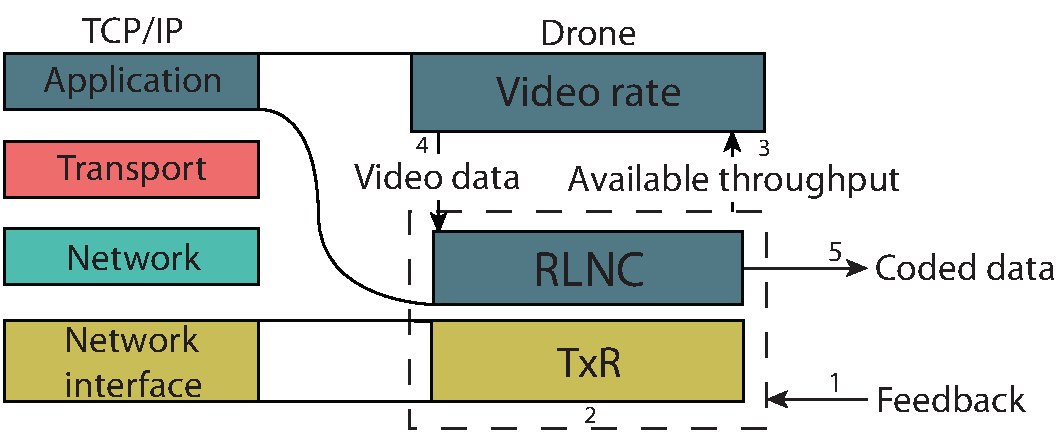
\includegraphics[scale=0.5]{images/TCP-Drone.pdf}
  \caption{The adjustment flow of reliable live video streaming and how the components relates to the TCP/IP stack.}
  \label{fig:usecase}
\end{figure}

The scenario examined is an open field where a drone captures live video and multicasts it to a number of receivers. The drone moves in an unpredictable pattern, but within a confined space of a circle with radius 100 m, where the receivers are placed in the center. For safety reasons the minimum hover height is 2 m. All receivers are located close together and within line of sight of the sender. Furthermore, it is assumed that all receivers have similar hardware and software configurations.


%At the receiver the video will be played back with a given \textit{playback delay} D.


%The environment of the system is an outdoor open field. Weather conditions might influence the amount of background noise, and nearby transmission equipment might be transmitting at the same frequency.

%assumptions
%We apply the following assumptions to the general systems presented in figure \ref{fig:usecasesimple}:
%\begin{itemize}
%\item The feedback from the receivers to the sender is perfect and instant
%\item Data rates can be changed instantaneously
%\item The only delay present in the video playback system is the delay caused by the transmission in the wireless link. (Network coding/decoding, video encoding, etc. does not cause delay).
%\item All receivers behave approximately identical to changes in positioning relative to the sender, i.e. have the same reception, have equal hardware etc.
%\item Packet error rate is an accurate measure of the channel condition, i.e. interference and signal fading is not differentiated
%\end{itemize}

%The primary performance metric of the system is the delay of the video stream. Depending on the actual application of the video stream, delay might have different severity. For a football match, you want a continuous video, which means delay might lead to buffering - and delayed playback. For a surveillance application immediate playback might be more desirable, and a delay might lead to jumps in the video. Common to both applications, the longest per frame delay is the critical factor for the performance of the system (the perception of the experience). For both cases it might be tolerable to have a constant delay of e.g. 500 ms. As long as the actual delay stays under the tolerable/standard delay, the video will appear smooth and clean. For this reason we evaluate the system based on the longest per frame delay. \textit{We could also evaluate the number of video rate changes at different "standard" delays e.g. 100 ms 200 ms, 500 ms and 1000 ms, and calculate the time at each video rate. - \textbf{this is out main contribution}}
%\begin{itemize}
%  \item introduce two ways of handling delay requirement (drop frames or switch)
%\end{itemize}
